\documentclass[12pt,a4paper]{article}

\usepackage[utf8]{inputenc}
\usepackage[T1]{fontenc}
\usepackage[english]{babel}
\usepackage{geometry}
\usepackage{listings}
\usepackage{xcolor}
\usepackage{float}
\usepackage{parskip}
\usepackage{fancyhdr}
\usepackage{booktabs}
\usepackage{tikz}
\usetikzlibrary{arrows.meta}
\usetikzlibrary{fit}

\geometry{margin=2cm}

\definecolor{codebg}{rgb}{0.95,0.95,0.95}
\definecolor{codegreen}{rgb}{0.1,0.5,0.1}
\definecolor{codegray}{rgb}{0.4,0.4,0.4}
\definecolor{codeblue}{rgb}{0.1,0.1,0.7}

\lstdefinelanguage{Erlang}{
  keywords={module,export,import,define,record,if,case,of,end,fun,receive,after,when,begin,try,catch,throw},
  keywordstyle=\color{codeblue}\bfseries,
  comment=[l]{\%},
  commentstyle=\color{codegreen}\itshape,
  stringstyle=\color{orange},
  morestring=[b]",
  sensitive=true
}

\lstset{
  language=Erlang,
  backgroundcolor=\color{codebg},
  basicstyle=\ttfamily\small,
  breaklines=true,
  frame=single,
  rulecolor=\color{gray},
  numbers=left,
  numberstyle=\tiny\color{codegray},
  tabsize=2,
  captionpos=b,
  showstringspaces=false,
  showspaces=false,
  showtabs=false
}

\pagestyle{fancy}
\fancyhf{}
\rhead{R-322 --- Operating Systems I}
\lhead{HPC Distributed Resource Manager}
\rfoot{Page \thepage}

\title{\textbf{HPC Distributed Resource Manager}\\[0.3em]\normalsize R-322 --- Operating Systems I}
\author{
Juan Ignacio Gorgo \\
Camila Sarasúa \\
Lucio Oviedo Dell'Orefice \\
Santiago Salvático
}
\date{June 23, 2026}
\usepackage{lmodern}
\begin{document}

\maketitle
\thispagestyle{fancy}
\tableofcontents
\newpage

%---------------------------------------------------------------
\section{Project Overview}

This report describes the design and implementation of a distributed resource manager
for a simulated HPC cluster. Each node consists of two cooperating components:
a \textbf{Resource Manager Agent} written in C, and a \textbf{Job Scheduler} written in Erlang.
The components communicate via TCP on localhost, while C agents communicate with each
other over the network using a common ASCII protocol.

The Erlang side is responsible for job generation, resource request orchestration,
deadlock prevention, and event logging. The C side manages local resources, handles
concurrent connections via \texttt{epoll}, and implements UDP-based node discovery.

%---------------------------------------------------------------
\section{Erlang Component Architecture}

\subsection{Module Overview}

The Erlang component is structured into four modules with clearly separated responsibilities:

\begin{center}
\begin{tabular}{ll}
\toprule
\textbf{Module} & \textbf{Responsibility} \\
\midrule
\texttt{header.hrl}         & Shared macros, records, and resource ordering constants \\
\texttt{erlang\_c\_bridge}  & TCP connection management with the local C agent \\
\texttt{job\_scheduler}     & Job generation, scheduling logic, and state management \\
\texttt{event\_logger}      & Asynchronous event logging to file \\
\bottomrule
\end{tabular}
\end{center}

\subsection{Process Architecture}

The system consists of two main components per node: a C agent and an Erlang scheduler.
The Erlang side uses the actor model --- each logical unit runs as an independent process communicating exclusively through message passing, with no shared memory.
The C agent handles all network I/O using \texttt{epoll}, delegating resource logic to internal modules connected through a well-defined interface.

\begin{figure}[H]{
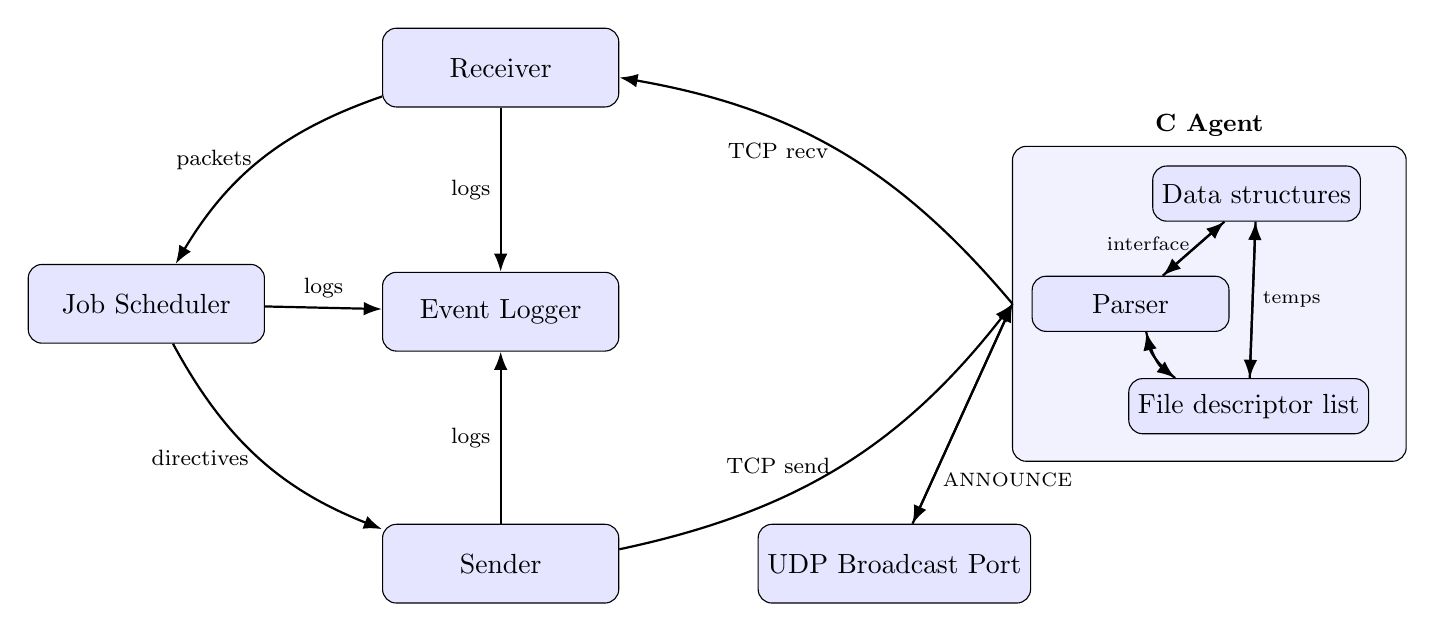
\begin{tikzpicture}[
  box/.style={
      draw=black,
      fill=blue!10,
      rounded corners=5pt,
      minimum width=3cm,
      minimum height=1cm,
      align=center
  },
  arr/.style={-{Latex}, thick}
]

\node[box] (receiver)   at (0,4)        {Receiver};
\node[box] (sched)      at (-4.5,1)     {Job Scheduler};
\begin{scope}[shift={(9,1)}]
  \draw[draw=black, fill=blue!5, rounded corners=5pt] 
    (-2.5,-2) rectangle (2.5,2);
  \node[above, font=\small\bfseries] at (0,2) {C Agent};
  
  \node[box, minimum width=2.5cm, minimum height=0.7cm] (datastr)    at (0.6, 1.4)  {Data structures};
  \node[box, minimum width=2.5cm, minimum height=0.7cm] (parser)   at (-1,0)  {Parser};
  \node[box, minimum width=2.5cm, minimum height=0.7cm] (fdlist)    at (0.5,-1.3)  {File descriptor list};

  \draw[arr] (parser)  -- node[left, font=\scriptsize, pos=0.6]{interface} (datastr);
  \draw[arr] (datastr)  -- (parser);
  \draw[arr] (datastr) -- node[right, font=\scriptsize]{temps} (fdlist);
  \draw[arr] (fdlist) -- (datastr);
  \draw[arr] (fdlist)  to[bend left=20] (parser);
  \draw[arr] (parser)  to[bend right=20] (fdlist);
\end{scope}

\coordinate (agent) at (6.5,1);
\node[box] (sender)     at (0,-2.3)     {Sender};
\node[box] (logger)     at (0,0.9)      {Event Logger};
\node[box] (udp)        at (5,-2.3)   	{UDP Broadcast Port};

\draw[arr] (sched) to[bend right=20] node[left, font=\footnotesize] {directives}  (sender);
\draw[arr] (receiver) to[bend right=20] node[left,font=\footnotesize] {packets}  (sched);
\draw[arr] (receiver) -- node[left, font=\footnotesize]{logs} (logger);
\draw[arr] (sched) -- node[above, font=\footnotesize] {logs} (logger);
\draw[arr] (sender) to[bend right=20] node[left, font=\footnotesize] {TCP send}   (agent);
\draw[arr] (sender) -- node[left, font=\footnotesize]{logs} (logger);
\draw[arr] (agent) to[bend right=20] node[left, font=\footnotesize] {TCP recv}   (receiver);
\draw[arr] (agent) -- node[right,font=\scriptsize, pos=0.8] {ANNOUNCE} (udp);
\draw[arr] (udp) -- (agent);


\end{tikzpicture}
}
\caption{System communication architecture: Erlang processes and C agent internals}
\end{figure}

\subsection{Test Environment Convention}

To simplify deadlock testing without the constraints of global resource ordering,
a \texttt{ENV} environment variable convention was introduced. When \texttt{ENV}
is set to \texttt{"test"}, the \texttt{generate\_job\_request} function skips
the resource sorting step, allowing jobs to request resources in arbitrary order.
This makes it possible to deliberately trigger the deadlock scenario described
in Section 4 and verify that the system detects or recovers from it.

In production (\texttt{ENV} unset or any other value), global ordering is always
applied and deadlock is structurally prevented.

\subsection{Startup Sequence}

\subsection{C Agent Startup Sequence}

The C agent is launched with five arguments: IP address, TCP port, and the 
available CPU, RAM, and GPU resources. The startup sequence is as follows:

\begin{enumerate}
    \item The \texttt{ServerContext} is initialized with the provided arguments and a new \texttt{epoll} instance is created.
    \item Three sockets are opened: a public TCP listener bound to the node's LAN IP, a local TCP listener bound to \texttt{127.0.0.1} exclusively 
 for the Erlang scheduler, and a UDP socket for broadcast discovery.
    \item Three \texttt{timerfd} instances are configured: a one-shot TCP timer (2 seconds), a periodic UDP announce timer (every 1 second), and a 
 periodic garbage collector timer (every 5 seconds).
    \item The three timers and the UDP socket are registered in epoll. The TCP sockets are intentionally \textbf{not} registered yet.
    \item A thread pool of 4 worker threads is initialized and begins waiting for tasks.
    \item The main epoll loop starts. During the first 2 seconds, only UDP traffic is processed — the node broadcasts its presence and collects     announcements from peers already on the network.
    \item When the TCP timer expires, both TCP sockets are added to epoll and the agent begins accepting connections from other agents and from the 
local Erlang scheduler.
\end{enumerate}
When \texttt{erlang\_c\_bridge:init/0} is called:

\begin{enumerate}
  \item Spawns the \texttt{event\_logger} process and registers it under the atom \texttt{eventLoggerId}.
  \item Spawns the \texttt{job\_scheduler} process.
  \item Calls \texttt{connect/3}, which attempts up to \texttt{?TRIES} TCP connections to the C agent.
  \item On success, spawns \texttt{conn\_handler}, which spawns \texttt{sender} and \texttt{receiver}
        and notifies the scheduler with their PIDs.
  \item On exhaustion of retries, logs the failure and calls \texttt{erlang:halt/0}.
\end{enumerate}

%---------------------------------------------------------------
\section{Communication Protocol}

\subsection{Inter-Agent Protocol (C to C)}

C agents communicate directly with each other over TCP using a line-oriented ASCII protocol, where each message is terminated by \texttt{\textbackslash n}. This protocol is used to reserve and release resources on remote nodes.

Messages sent between agents:

\begin{lstlisting}
RESERVE <job_id> <resource_name> <amount>
GRANTED <job_id>
DENIED  <job_id>
RELEASE <job_id> <resource_name> <amount>
\end{lstlisting}

Where \texttt{job\_id} is a unique integer generated by the Erlang scheduler,
\texttt{resource\_name} is one of \texttt{cpu}, \texttt{mem}, or \texttt{gpu},
and \texttt{amount} is the requested quantity.

Node discovery is handled via UDP broadcast. Each agent periodically announces
its presence with:

\begin{lstlisting}[language={}]
ANNOUNCE <port> <cpu:N> <mem:N> <gpu:N>
\end{lstlisting}

The sender's IP is extracted directly from \texttt{recvfrom()} rather than
included in the message. If no announcement is received from a node within
15 seconds, it is considered dead and removed from the known nodes table.

\subsection{Local Interface (Erlang to C Agent)}

The \texttt{sender} process forwards directives from the scheduler to the C agent:

\begin{lstlisting}
GET_NODES
JOB_REQUEST <job_id> @<ip>:<port>:<resource>:<amount> ...
JOB_RELEASE <job_id>
\end{lstlisting}

The \texttt{receiver} process listens on the same socket and forwards responses to the scheduler:

\begin{lstlisting}
NODES <ip>:<port>:<res>:<amount>:...;<ip>:...
JOB_GRANTED <job_id>
JOB_DENIED  <job_id>
JOB_TIMEOUT <job_id>
\end{lstlisting}

\subsection{Sequence Diagram: Successful Job Lifecycle}

\begin{figure}[H]
\centering
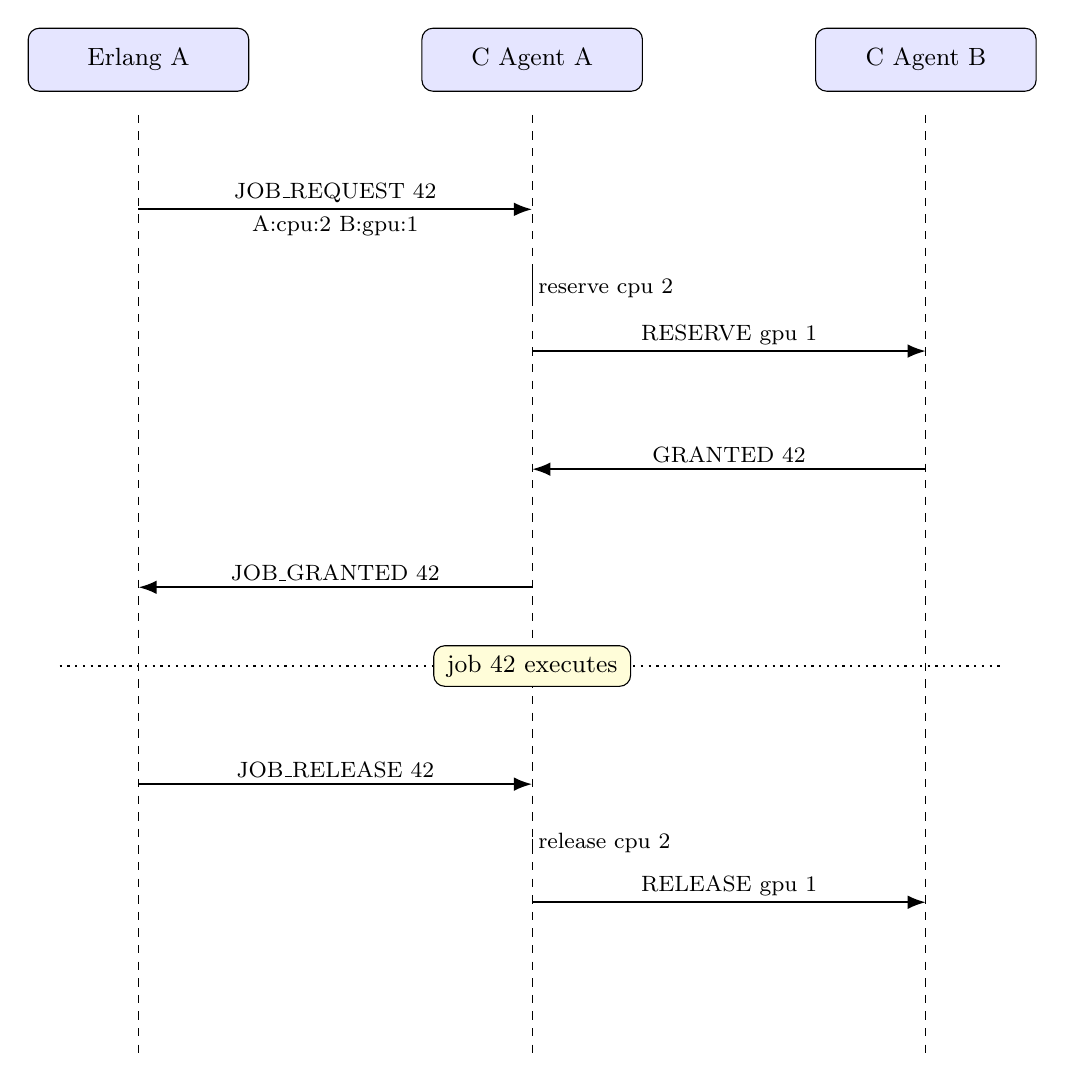
\begin{tikzpicture}[
    font=\small,
    proc/.style={
        draw,
        rounded corners,
        fill=blue!10,
        minimum width=2.8cm,
        minimum height=0.8cm
    },
    msg/.style={
        font=\footnotesize,
        inner sep=2pt
    },
    arr/.style={
        -{Latex},
        thick
    }
]

% Participants
\node[proc] (ea) at (0,0.7) {Erlang A};
\node[proc] (ca) at (5,0.7) {C Agent A};
\node[proc] (cb) at (10,0.7) {C Agent B};

% Lifelines
\foreach \x in {0,5,10}
    \draw[dashed] (\x,0) -- (\x,-12);

% Job request
\draw[arr]
    (0,-1.2) --
    node[msg,above]
    {JOB\_REQUEST 42}
    node[msg,below]{A:cpu:2 B:gpu:1}
    (5,-1.2);

% Local reservation
\draw[dashed]
    (5,-2) --
    node[msg,right]
    {reserve cpu 2}
    (5,-2.4);

% Remote reservation
\draw[arr]
    (5,-3) --
    node[msg,above]
    {RESERVE gpu 1}
    (10,-3);

% Grant
\draw[arr]
    (10,-4.5) --
    node[msg,above]
    {GRANTED 42}
    (5,-4.5);

% Notify Erlang
\draw[arr]
    (5,-6) --
    node[msg,above]
    {JOB\_GRANTED 42}
    (0,-6);

% Separator
\draw[dotted, thick]
    (-1,-7) -- (11,-7);

\node[
    draw,
    rounded corners,
    fill=yellow!15,
    minimum width=2.5cm
]
at (5,-7)
{job 42 executes};

% Release
\draw[arr]
    (0,-8.5) --
    node[msg,above]
    {JOB\_RELEASE 42}
    (5,-8.5);

% Local release
\draw[dashed]
    (5,-9.2) --
    node[msg,right]
    {release cpu 2}
    (5,-9.3);

% Remote release
\draw[arr]
    (5,-10) --
    node[msg,above]
    {RELEASE gpu 1}
    (10,-10);

\end{tikzpicture}

\caption{Successful job execution and release.}
\end{figure}
\newpage
%---------------------------------------------------------------
\section{Deadlock Prevention Strategy}

\subsection{Problem Description}

Distributed deadlock occurs when two jobs each hold a resource the other needs,
forming a circular wait. The classic scenario from the assignment:

\begin{itemize}
  \item \textbf{Job1} (from Node A): needs 2 CPUs from Node A and 1 GPU from Node B.
  \item \textbf{Job2} (from Node B): needs 1 GPU from Node B and 2 CPUs from Node A.
\end{itemize}

If both jobs acquire their first resource simultaneously, each blocks waiting
for the resource held by the other - a deadlock.

\subsection{Strategy: Global Resource Ordering}

The chosen strategy eliminates the \textbf{circular wait} condition (Coffman condition 4)
by enforcing a global ordering on all resource requests before sending them.

Before sending a \texttt{JOB\_REQUEST}, the scheduler sorts the list of required resources
by the pair \texttt{(NodeIp, ResourceType)} in ascending order. The type order is
defined centrally in \texttt{header.hrl}:

\begin{lstlisting}
-define(RES_ORDER(Type),
    case Type of
        cpu -> 1;
        ram -> 2;
        gpu -> 3
    end
).
\end{lstlisting}

The sort is applied in \texttt{generate\_job\_request/2}:

\begin{lstlisting}
SortedResources = lists:sort(
    fun ({Ip1, Resource1, _}, {Ip2, Resource2, _}) ->
        {Ip1, Resource1} =< {Ip2, Resource2}
    end,
    AvailableResources
),
\end{lstlisting}

\subsection{Why This Works: Step-by-Step Example}

With the ordering invariant enforced, the deadlock scenario resolves as follows:

\begin{enumerate}
  \item Both Job1 and Job2 sort their resource lists. Since \texttt{"A" < "B"}
        lexicographically, both lists start with resources from Node A.
  \item Both jobs compete for Node A's CPUs first. One wins; the other waits
        in Node A's FIFO queue.
  \item The winning job (Job1) then requests Node B's GPU and acquires it.
  \item Job1 finishes, releases both resources. Job2 then acquires Node A's CPUs,
        then Node B's GPU, and completes normally.
\end{enumerate}

The key invariant: \textit{no job can hold a resource from a ``later'' node while
waiting for a resource from an ``earlier'' node.} Circular wait is structurally
impossible.

%---------------------------------------------------------------
\section{Event Logger}

\subsection{Design}

The logger runs as a dedicated Erlang process, registered under the atom
\texttt{eventLoggerId}. Any module logs an event by calling:

\begin{lstlisting}
event_logger:log_event(Status, SrcMethod, Detail, JobInvolved)
\end{lstlisting}

This builds a \texttt{\#logInfo\{\}} record and sends it as a message to the logger,
which writes it to \texttt{event\_logger.txt} in append mode using \texttt{raw} file I/O.

\subsection{Log Record}

\begin{lstlisting}
-record(logInfo, {
    status,       % ok | error | close
    src_method,   % {Module, Function}
    detail,       % atom | string describing the event
    job_involved, % job_id integer | none
    timestamp     % {Hour, Min, Sec}
}).
\end{lstlisting}

\subsection{Example Output}

\begin{lstlisting}
ok {erlang_c_bridge,init} initialization none {14,32,10}
ok {erlang_c_bridge,connect} "CONNECTION SUCCESSFUL" none {14,32,10}
ok {job_scheduler,init} "[job_scheduler] sender_pid received" none {14,32,11}
ok {job_scheduler,init} "[job_scheduler] job_request" 5 {14,32,16}
ok {job_scheduler,init} "[job_scheduler] job_granted" 5 {14,32,16}
\end{lstlisting}

\subsection{Design Rationale}

Registering the logger under a fixed atom avoids threading the logger PID
through every function call. Any process in the system can log at any time
without holding a reference.

%---------------------------------------------------------------
\section{Team Contributions}

\begin{center}
\begin{tabular}{ll}
\toprule
\textbf{Member} & \textbf{Contributions} \\
\midrule
{[Lucio Oviedo Dell'Orefice]} & C Agent: epoll server, TCP handling, non-blocking I/O. \\\\
{[Juan Ignacio Gorgo]} & C Agent: resource management, FIFO queues,\\
			& GRANTED/DENIED logic. \\\\
{[Camila Sarasúa]} & Erlang: job scheduler, deadlock prevention, job state machine. \\\\
{[Santiago Salvático]} & Erlang: \texttt{erlang\_c\_bridge}, \texttt{event\_logger}, \\
             & \texttt{header.hrl}, documentation, integration. \\
\bottomrule
\end{tabular}
\end{center}

\section{Implementation Challenges}

During the development of the distributed resource manager, several implementation issues were identified and resolved. These problems influenced both the communication protocol and the internal architecture of the system.

\subsection{Agent Identification}

Initially, C agents were identified solely by their IP address. This approach proved insufficient when multiple agents were executed on the same host, since different nodes could share the same IP while listening on different ports.

To solve this issue, agents were uniquely identified using the pair:

\begin{center}
\texttt{(IP, Port)}
\end{center}

This identifier became part of node discovery, remote communication, and resource allocation messages, allowing multiple agents to coexist on the same machine.

\subsection{Remote Resource Ownership}

As the system evolved to support multiple agents, resources could belong to different nodes. A job request might require resources distributed across several machines.

For this reason, resource descriptors were extended to include the destination node information. Reservation and release operations therefore target the correct remote agent, ensuring that resources are allocated and released consistently.

\subsection{Parser Interoperability Between C and Erlang}

Communication between the C agent and the Erlang scheduler exposed several interoperability issues.

Initially, some messages generated by the C agent contained trailing newline characters. When Erlang attempted to convert values such as:

\begin{lstlisting}
"1\n"
\end{lstlisting}

directly into integers, parsing failures occurred.

The Erlang parser was modified to normalize incoming fields using \texttt{string:trim/1} before converting values, improving robustness against formatting differences.

\subsection{UDP Discovery Traffic}

The distributed discovery mechanism relies on periodic UDP announcements between agents.

Early versions used a very short announcement interval, producing unnecessary network traffic and excessive log output. In addition, incorrect startup parameters occasionally caused invalid announcement messages.

The discovery protocol was stabilized by increasing the broadcast interval and standardizing the announcement format:

\begin{lstlisting}
ANNOUNCE <port> cpu:<cpu> mem:<memory> gpu:<gpu>
\end{lstlisting}

This reduced network noise while maintaining reliable node discovery.

%---------------------------------------------------------------
\section{Problems Encountered and Solutions}

\subsection{Job ID Collision Between Nodes on the Same IP}

\textbf{Problem:} The assignment specifies that two nodes may share the same IP address as long as they use different ports. Since each node's Erlang scheduler generates job IDs independently using \texttt{erlang:unique\_integer/1}, two schedulers on the same IP can produce identical job IDs. When a third agent receives a \texttt{RESERVE 42 cpu 2} message, it cannot determine which node
sent it based on the job ID alone.

\textbf{Solution:} The C agent already has access to the file descriptor (\texttt{fd}) of the incoming TCP connection via the \texttt{SOCKET} parameter in \texttt{resource\_adapter\_patch}. Since the kernel guarantees that no two active connections share the same \texttt{fd} within a process, the pair \texttt{(job\_id, fd)} is globally unique:

\begin{itemize}
    \item \texttt{fd} uniquely identifies which node sent the message.
    \item Within the same connection (\texttt{fd}), \texttt{erlang:unique\_integer} guarantees the job ID never repeats.
\end{itemize}

The solution required no changes to the network protocol — the \texttt{fd} is already available throughout the event handling pipeline and only needed to be incorporated as part of the job key in the active jobs table.

\subsection{Early Closing Socket}

\textbf{Problem:} When the process that opened a TCP socket exits, Erlang closes
the socket automatically. This caused the connection to drop when \texttt{conn\_handler}
spawned children and then terminated.

\textbf{Solution:} The socket ID is passed directly to processes \texttt{sender} and \texttt{receiver} at spawn time. Since these are long-lived processes, the socket remains open for the session's duration.

\subsection{Logger Process Id Registration}

\textbf{Problem:} Passing the logger PID through every function call created
unnecessary coupling between modules.

\textbf{Solution:} The logger is registered under the atom \texttt{eventLoggerId}
via \texttt{register/2}. All modules send log messages to the atom directly.

\subsection{TCP Read Blocking vs.\ Erlang Message Passing}

\textbf{Problem:} A process blocked in \texttt{gen\_tcp:recv} with \texttt{\{active, false\}} cannot receive Erlang messages simultaneously.
The alternative, \texttt{\{active, true\}}, delivers TCP data directly to the process mailbox --- but if the C agent sends messages faster than the process consumes them, the mailbox can exhaust memory.

\textbf{Solution:} We kept \texttt{\{active, false\}} and separated inbound and onbound traffic into two dedicated processes:
\begin{itemize}
\item \texttt{receiver:} blocks on \texttt{gen\_tcp:recv} waiting for C agent responses.
\item \texttt{sender:  } blocks on \texttt{receive} waiting for scheduler directives.
\end{itemize}
Each process has a single blocking responsibility, avoiding both problems.

\end{document}
